\documentclass[journal,12pt,twocolumn]{IEEEtran}

\usepackage{setspace}
\usepackage{gensymb}

\singlespacing

\usepackage[cmex10]{amsmath}
\usepackage{amsthm}
\usepackage{mathrsfs}
\usepackage{txfonts}
\usepackage{stfloats}
\usepackage{bm}
\usepackage{cite}
\usepackage{cases}
\usepackage{subfig}
\usepackage{longtable}
\usepackage{multirow}
\usepackage{mathtools}
\usepackage{steinmetz}
\usepackage{tikz}
\usepackage{circuitikz}
\usepackage{verbatim}
\usepackage{tfrupee}
\usepackage[breaklinks=true]{hyperref}
\usepackage{tkz-euclide} % loads  TikZ and tkz-base
%\usetkzobj{all}
\usetikzlibrary{calc,math}
\usepackage{listings}
    \usepackage{color}                                            %%
    \usepackage{array}                                            %%
    \usepackage{longtable}                                        %%
    \usepackage{calc}                                             %%
    \usepackage{multirow}                                         %%
    \usepackage{hhline}                                           %%
    \usepackage{ifthen}                                           %%
  %optionally (for landscape tables embedded in another document): %%
    \usepackage{lscape}    
\usepackage{graphicx}
\usepackage{multicol}
\usepackage{chngcntr}
\DeclareMathOperator*{\Res}{Res}
\renewcommand\thesection{\arabic{section}}
\renewcommand\thesubsection{\thesection.\arabic{subsection}}
\renewcommand\thesubsubsection{\thesubsection.\arabic{subsubsection}}

\renewcommand\thesectiondis{\arabic{section}}
\renewcommand\thesubsectiondis{\thesectiondis.\arabic{subsection}}
\renewcommand\thesubsubsectiondis{\thesubsectiondis.\arabic{subsubsection}}

\newcommand{\bignorm}[1]{\Bigl \| #1 \Bigr \| #1}
\newcommand{\norm}[1]{\| #1 \|}
% correct bad hyphenation here
\hyphenation{op-tical net-works semi-conduc-tor}
\def\inputGnumericTable{}                                 %%

\lstset{
frame=single, 
breaklines=true,
columns=fullflexible
}


\begin{document}
\begin{center}
\huge Assignment 2\\

\large Shaik Zeeshan Ali\\
\large AI20MTECH11001\\
\end{center}
\vspace{0.5cm}
\begin{abstract}
This document explains how to find the shortest distance between two lines if and when the two lines are not intersecting with each other.
\end{abstract}
\vspace{0.5cm}
Download all python codes from 
\begin{lstlisting}
https://github.com/Zeeshan-IITH/IITH-EE5609/new/master/codes
\end{lstlisting}
%
and latex-tikz codes from 
\begin{lstlisting}
https://github.com/Zeeshan-IITH/IITH-EE5609
\end{lstlisting}
%
\vspace{0.5cm}
\section{Problem}
Find the shortest distance between the lines \\
\begin{align}
    L_1\colon \bm{x}= \begin{pmatrix}1\\2\\1\end{pmatrix}+\lambda_1\begin{pmatrix}1\\-1\\1\end{pmatrix}\\
    L_2\colon \bm{x}= \begin{pmatrix}2\\-1\\-1\end{pmatrix}+\lambda_2\begin{pmatrix}2\\1\\2\end{pmatrix}
\end{align}
\section{construction}
When two lines are not intersecting the distance between them is non-zero.The equation of above mentioned lines in symmetric form is
\begin{align}
    L_1\colon x-1=2-y=z-1\\
    L_2\colon \frac{x-2}{2}=y+1=\frac{z+1}{2}
\end{align}
The above line equations have no point of intersection as for no value of $\lambda_1,\lambda_2$ both the equations (3) and (4) are equal.\par
If the two line intersect then (3)=(4) i.e.
\begin{align}
    \begin{pmatrix}1\\2\\1\end{pmatrix}+\lambda_1\begin{pmatrix}1\\-1\\1\end{pmatrix}=\begin{pmatrix}2\\-1\\-1\end{pmatrix}+\lambda_2\begin{pmatrix}2\\1\\2\end{pmatrix}\\
    \lambda_1\begin{pmatrix}1\\-1\\1\end{pmatrix}-\lambda_2\begin{pmatrix}2\\1\\2\end{pmatrix}=\begin{pmatrix}1\\-3\\-2\end{pmatrix}\\
    \begin{pmatrix}1 & -2\\-1 & -1\\1 & -2\end{pmatrix}\begin{pmatrix}\lambda_1\\\lambda_2\end{pmatrix}=\begin{pmatrix}1\\-3\\-2\end{pmatrix}\\
    \intertext{The Augmented matrix will be}\\
    \begin{pmatrix}1 & -2 & 1\\-1 & -1 & -3\\1 & -2 & -2\end{pmatrix}\\
    \begin{pmatrix}1 & -2 & 1\\-1 & -1 & -3\\1 & -2 & -2\end{pmatrix}\underleftrightarrow{R_1=R_1-R_2}\begin{pmatrix}0 & 0 & 3\\-1 & -1 & -3\\1 & -2 & -2\end{pmatrix}
\end{align}
The above matrix has a $rank=3$ .Hence the lines do not intersect
\section{solution}
Let $\bm{A}$ be a point on line $L_1$ and $\bm{B}$ be point on the line $L_2$.Then the shortest distance between two skew lines will be the length of line perpendicular to both the lines $L_1$,$L_2$ and passing through $\bm{A}$ and $\bm{B}$.\par
\vspace{5mm}
The vector passing through $\bm{A}$ and $\bm{B}$ will be \\
\begin{align}
    \bm{A-B}=\bm{x_1-x_2}+\begin{pmatrix}\bm{m_1} & -\bm{m_2}\end{pmatrix}\begin{pmatrix}\lambda_1\\\lambda_2\end{pmatrix}
\end{align}
The vectors $\bm{m_1}$,$\bm{m_2}$ are both perpendicular to the line $\bm{AB}$.So the dot product of $\bm{m_1}$,$\bm{m_2}$ with the line $\bm{AB}$ is zero.\\

The dot product of $\bm{m_1}$ with the line $\bm{AB}$ is
\begin{align}
    \bm{m_1}^T(\brak\bm{A-B})=0\notag\\
    \bm{m_1^T}(\bm{x_1-x_2})+\bm{m_1^T}(\bm{m_1} & -\bm{m_2})\begin{pmatrix}\lambda_1 \\ \lambda_2\end{pmatrix}=0
\end{align}
The dot product of $\bm{m_2}$ with the line $\bm{AB}$ is\\
\begin{align}
    \bm{m_2}^T(\brak\bm{A-B})=0\notag\\
    \bm{m_1^T}(\bm{x_1-x_2})+\bm{m_2^T}(\bm{m_1} & -\bm{m_2})\begin{pmatrix}\lambda_1 \\ \lambda_2\end{pmatrix}=0
\end{align}
\vspace{3mm}
Combining the equations $(12)$ and $(13)$ in matrix form we get\\
\begin{align}
    \begin{pmatrix}\bm{m_1^T}\bm{m_1} & -\bm{m_1^T}\bm{m_2}\\\bm{m_2^T}\bm{m_1} &  -\bm{m_2^T}\bm{m_2}\end{pmatrix}\begin{pmatrix}\lambda_1\\\lambda_2\end{pmatrix}+\begin{pmatrix}\bm{m_1^T}\bm{(x_1-x_2)}\\\bm{m_2^T}\bm{(x_1-x_2)}\end{pmatrix}=0
\end{align}
simplifying it further\\
\begin{align}
    \begin{pmatrix}\bm{m_1^T}\bm{m_1} & -\bm{m_1^T}\bm{m_2}\\\bm{m_2^T}\bm{m_1} &  -\bm{m_2^T}\bm{m_2}\end{pmatrix}\begin{pmatrix}\lambda_1\\\lambda_2\end{pmatrix}=\begin{pmatrix}\bm{m_1^T}\bm{(x_2-x_1)}\\\bm{m_2^T}\bm{(x_2-x_1)}\end{pmatrix}
\end{align}
To find the points on the lines which make up the shortest distance we need to find $\lambda_1$ and $\lambda_2$ using the following expression\\
\begin{align}
    \begin{pmatrix}\bm{m_1^T}\bm{m_1} & -\bm{m_1^T}\bm{m_2}\\\bm{m_2^T}\bm{m_1} &  -\bm{m_2^T}\bm{m_2}\end{pmatrix}\begin{pmatrix}\lambda_1\\\lambda_2\end{pmatrix}=\begin{pmatrix}\bm{m_1^T}\bm{(x_2-x_1)}\\\bm{m_2^T}\bm{(x_2-x_1)}\end{pmatrix}\\
    \intertext{we know that\notag\\}
    \bm{x_1}=\begin{pmatrix}1\\2\\1\end{pmatrix},\bm{x_2}=\begin{pmatrix}2\\-1\\-1\end{pmatrix},\bm{m_1}=\begin{pmatrix}1\\-1\\1\end{pmatrix} and  \bm{m_2}=\begin{pmatrix}2\\1\\2\end{pmatrix}\notag
\end{align}
Using the above expression, we get the points as $\frac{1}{12}\begin{pmatrix}27\\-3\\27\end{pmatrix}$ and $\frac{1}{12}\begin{pmatrix}10\\-19\\-26\end{pmatrix}$ on the line $L_1$,$L_2$ respectively.\\
The shortest distance between the lines is the absolute value of projection of the vector $\bm{AB}$ on to the unit vector $\bm{u}$.
\begin{equation}
    \norm{(\bm{B}-\bm{A})}\\
    =\norm{\frac{1}{{12}}\begin{pmatrix}27\\-3\\27\end{pmatrix}-\frac{1}{{12}}\begin{pmatrix}10\\-19\\-26\end{pmatrix}}\\
    =\frac{3}{\sqrt{2}}
\end{equation}
Therefore the shortest distance between the given lines is $\frac{3}{\sqrt{2}}$\\
The unit vector perpendicular to lines \\
\begin{align}
    Line_1\colon \bm{x}=\bm{x_1}+\lambda_1\bm{m_1}\\
    Line_2\colon \bm{x}=\bm{x_2}+\lambda_1\bm{m_2}
\end{align}
can be found by 
\begin{align}
    \frac{\frac{1}{{12}}\begin{pmatrix}27\\-3\\27\end{pmatrix}-\frac{1}{{12}}\begin{pmatrix}10\\-19\\-26\end{pmatrix}}{\norm{\frac{1}{{12}}\begin{pmatrix}27\\-3\\27\end{pmatrix}-\frac{1}{{12}}\begin{pmatrix}10\\-19\\-26\end{pmatrix}}}
\end{align}
So the unit vector perpendicular to both $L_1$ and $L_2$ is
\begin{align}
    \bm{n}=\frac{1}{\sqrt{2}}\begin{pmatrix}-1\\0\\1\end{pmatrix}
\end{align}

\begin{center}
    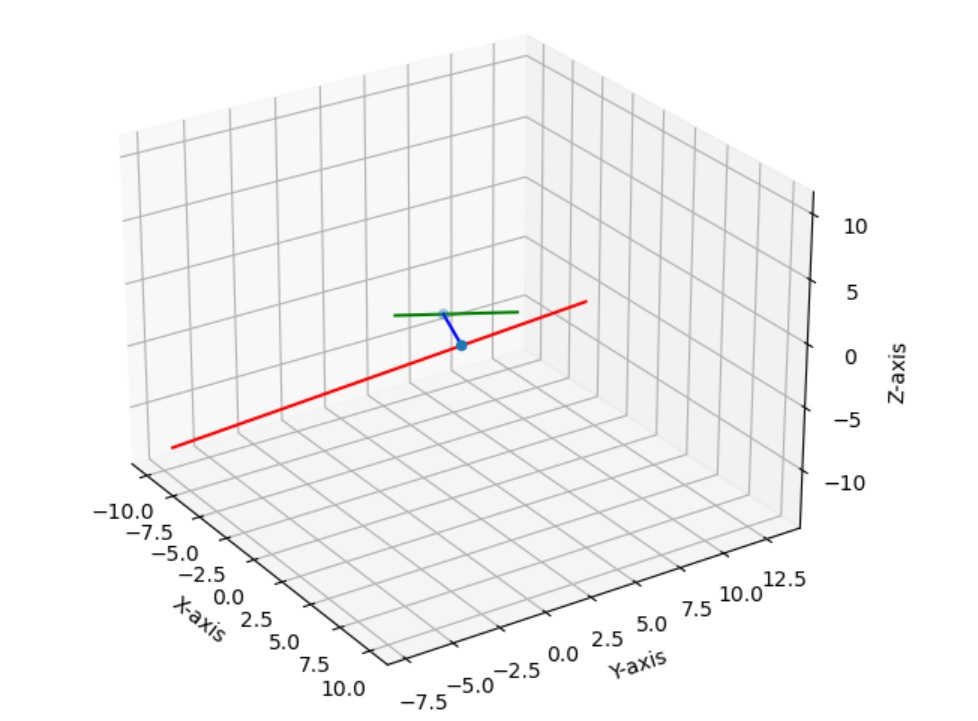
\includegraphics[width=11cm]{assignment2.jpg}
\end{center}
\end{document}
